\documentclass[tikz,border=2mm]{standalone}

\usetikzlibrary{arrows,positioning}

\begin{document}

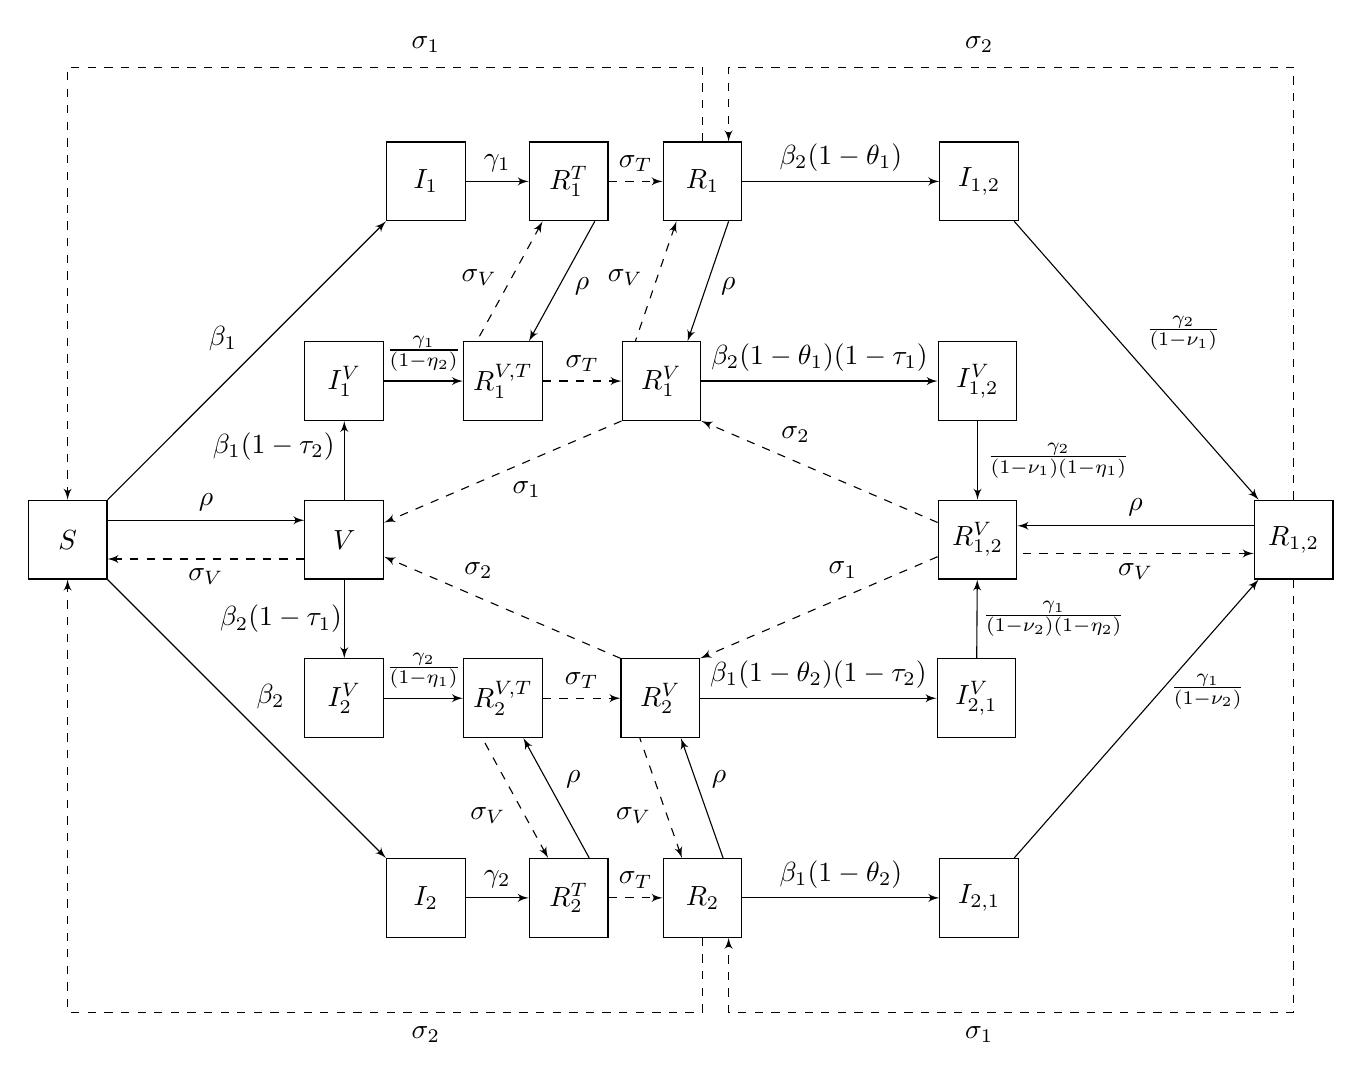
\begin{tikzpicture}[node distance=2.5cm,auto,>=latex',every node/.append style={align=center},int/.style={draw, minimum size=1cm},inverter/.style={rectangle,draw,inner sep=2pt,minimum size=6mm},]
    \node [int] (S)                                    {$S$};
    \node [int, above right=5cm of S] (I1)             {$I_1$};
    \node [int, below right=5cm of S] (I2)             {$I_2$};
    \node [int, right=of I1] (R1)             {$R_1$};
    \node [int, right=of I2] (R2)             {$R_2$};
    \node [int, right=of R1] (I12)             {$I_{1,2}$};
    \node [int, right=of R2] (I21)             {$I_{2,1}$};
    
    \path[->] (S) edge node {$\beta_1$} (I1);
    \path[->] (S) edge node {$\beta_2$} (I2);
    \path[->] (R1) edge node {$\beta_2(1-\theta_1)$} (I12);
    \path[->] (R2) edge node {$\beta_1(1-\theta_2)$} (I21);
    \node [int, right=of S] (V)                       {$V$};
    \node [int, below=1cm of V] (IV2)               {$I^V_2$};
    \node [int, right=1cm of IV2] (RVT2)              {$R^{V,T}_2$};
    \node [int, right=3cm of IV2] (RV2)               {$R^V_2$};
    % \node [int, right=of I12] (RT12)                   {$R^T_{1,2}$};
    \node [int, above=1cm of V] (IV1)                 {$I^V_1$};
    \node [int, right=1cm of IV1](RVT1)               {$R^{V,T}_1$};
    \node [int, right=1cm of RVT1] (RV1)              {$R^V_1$};
    \node [int, right=3cm of RV1] (IV12)              {$I^V_{1,2}$};
    
    
    \node [int, below=1cm of IV12] (RV12)                {$R^V_{1,2}$};
    \node [int, right=3cm of RV12] (R12)             {$R_{1,2}$};
    \path [->,dashed] (RV1.south west) edge node {$\sigma_1$} (V);
    \path [->,dashed] (RV2.north west) edge node [yshift=0.7cm] {$\sigma_2$} (V);
    
    \node [int, right=3cm of RV2] (IV21)                 {$I^V_{2,1}$};
    \path [->] (V) edge node [yshift=5pt] {$\beta_1(1-\tau_2)$} (IV1);
    \path [->] (V) edge node [xshift=-1.7cm] {$\beta_2(1-\tau_1)$} (IV2);
    \path [->] (IV1) edge node {$\frac{\gamma_1}{(1-\eta_2)}$} (RVT1);
    \path [->] (IV2) edge node {$\frac{\gamma_2}{(1-\eta_1)}$} (RVT2);
    \path [->,dashed] (RVT2) edge node {$\sigma_T$} (RV2);
    \path [->] (RV1) edge node {$\beta_2(1-\theta_1)(1-\tau_1)$} (IV12);
    \path [->] (IV12) edge node {$\frac{\gamma_2}{(1-\nu_1)(1-\eta_1)}$} (RV12);
    \path [->] (IV21) edge node [xshift=2cm] {$\frac{\gamma_1}{(1-\nu_2)(1-\eta_2)}$} (RV12);
    
    \path [->] (RV2) edge node {$\beta_1(1-\theta_2)(1-\tau_2)$} (IV21);
    \path ([yshift=7pt] S.east) edge [->] node {$\rho$} ([yshift=7pt] V.west)
    ([yshift=-7pt] V.west) edge [->,dashed] node {$\sigma_V$} ([yshift=-7pt] S.east);
    \path ([yshift=5pt] RV12.east) edge [<-] node {$\rho$} ([yshift=5pt] R12.west)
    ([yshift=-5pt] R12.west) edge [<-,dashed] node {$\sigma_V$} ([yshift=-5pt] RV12.east);
    \path ([xshift=-7pt] RV2.south east) edge [<-] node {$\rho$} ([xshift=-7pt] R2.north east)
    ([xshift=7pt] R2.north west) edge [<-,dashed] node {$\sigma_V$} ([xshift=7pt] RV2.south west);
    \path ([xshift=-5pt] RV1.north east) edge [<-] node [xshift=-20pt,yshift=-5pt] {$\sigma_V$} ([xshift=-5pt] R1.south east)
    ([xshift=5pt] R1.south west) edge [<-,dashed] node [xshift=20pt,yshift=5pt] {$\rho$} ([xshift=5pt] RV1.north west);
    
    
    \draw[->, auto=false, dashed] (R1.north) |- (6,6) -| (S.north);
    \draw[->, auto=false, dashed] (R2.south) |- (0,-6) -| (S.south);
    \node[below= 1cm of I2] (sigma2) {$\sigma_2$};
    \node[above= 1cm of I1] (sigma1) {$\sigma_1$};
    
    \path [->,dashed] (RV12) edge node [yshift=20pt] {$\sigma_2$} (RV1.south east);
    \path [->,dashed] (RV12) edge node [yshift=20pt] {$\sigma_1$} (RV2.north east);
    %strain-transcending immunity
    \node[int, right=0.8cm of I2] (RT2) {$R^T_2$};
    \node[int, right=0.8cm of I1] (RT1) {$R^T_1$};
    
    \path[->] (I12) edge node {$\frac{\gamma_2}{(1-\nu_1)}$} (R12);
    \path[->] (I21) edge node [xshift=1.5cm] {$\frac{\gamma_1}{(1-\nu_2)}$} (R12);
    % \path[->,dashed] (RT12) edge node {$\sigma_T$} (R12);
    % \draw[->] (I21.east) -| (17,0) |- (RT12.east);
    % \node[below right=1.9cm of IV21] (gamma21) {$\frac{\gamma_1}{(1-\nu_2)}$};
    \path[->] (I1) edge node {$\gamma_1$} (RT1);
    \path[->] (I2) edge node {$\gamma_2$} (RT2);
    \path[->,dashed] (RT1) edge node {$\sigma_T$} (R1);
    \path[->,dashed] (RT2) edge node {$\sigma_T$} (R2);
    \path[->,dashed] (RVT1) edge node {$\sigma_T$} (RV1);
    
    \draw[->,dashed] (R12.north) |-(9,6)-| ([xshift=-5pt] R1.north east);
    \draw[->,dashed] (R12.south) |-(9,-6)-| ([xshift=-5pt] R2.south east);
    \node[below= 1cm of I21] (sigma11) {$\sigma_1$};
    \node[above= 1cm of I12] (sigma22) {$\sigma_2$};
    \path ([xshift=-5pt] RVT1.north east) edge [<-] node [xshift=-20pt,yshift=-5pt] {$\sigma_V$} ([xshift=-5pt] RT1.south east)
    ([xshift=5pt] RT1.south west) edge [<-,dashed] node [xshift=20pt,yshift=5pt] {$\rho$} ([xshift=5pt] RVT1.north west);
    \path ([xshift=-7pt] RVT2.south east) edge [<-] node {$\rho$} ([xshift=-7pt] RT2.north east)
    ([xshift=7pt] RT2.north west) edge [<-,dashed] node {$\sigma_V$} ([xshift=7pt] RVT2.south west);
\end{tikzpicture}
\end{document}
